\chapter{Języki i~metody programowania}
\PartialToc
%\startcontents[chapters]
%\printcontents[chapters]{}{1}{\section*{\contentsname}}
\section{IT1A\_W03,IT1A\_U03,IT1A\_U07}
\textbf{W~jaki sposób można obliczyć długość tekstu przekazanego jako argument w~poniższej funkcji?}
\begin{lstlisting}[language=c]
void foo(const char* txt) {
. . .
}
\end{lstlisting}
\subsection{Odpowiedź}

\begin{itemize}
\item Używając funkcji strlen z biblioteki string.h
\begin{lstlisting}[language=c]
/* Declaration */
size_t strlen(const char *str)

/* Example */
strlen(txt)
\end{lstlisting}

\item Zliczając ile znaków występuje w tekście od znaku na który wskazuje wskaźnik do znaku końca łańcucha znaków ('\textbackslash0')
\begin{lstlisting}[language=c]
int length = 0;
char c = *txt;
while(c != '\0') {
   length++;
   c = *(++txt);
}
\end{lstlisting}
\end{itemize}
  
\subsection{Wprowadzenie teoretyczne}
\textbf{Łańcuch znaków}\\
Łańuch znaków w języku C to tablica znaków której ostatni element ma wartość \textbackslash0 - null\\
Poniższe deklaracje łańcucha znaków są równoważne:
\begin{lstlisting}[language=c]
char greeting[]  = "Hello";
char greeting[6] = "Hello";
char *greeting   = "Hello";
char greeting[]  = { 'H', 'e', 'l', 'l' 'o', '\0'};
char greeting[6] = { 'H', 'e', 'l', 'l' 'o', '\0'};
\end{lstlisting}

\begin{center}
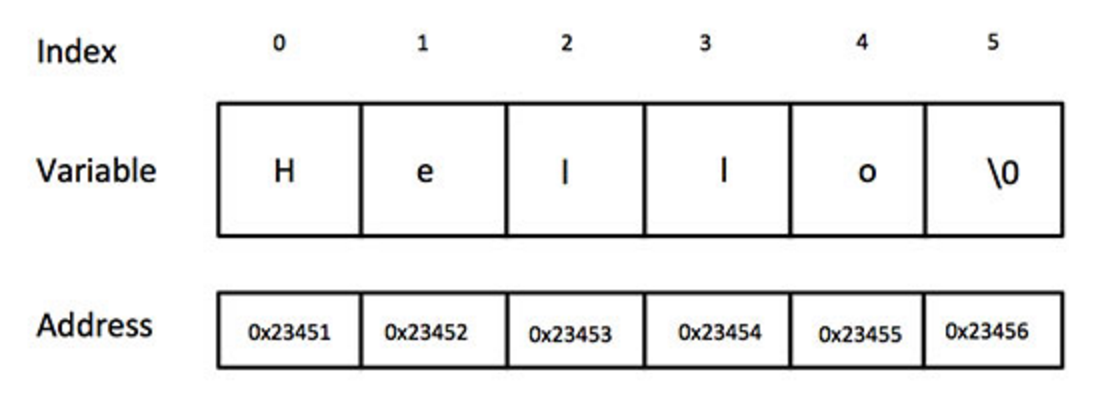
\includegraphics[width=13cm]{string_in_c}
\captionof{figure}{Łańcuchy znaków w C}
\end{center}

Istnieje biblioteka string.h która zawiera funkcja ułatwiające manipulowanie łańcuchami znaków.
\begin{lstlisting}[language=c]
strcpy(s1, s2); 
/*Copies string s2 into string s1*/

strcat(s1, s2);
/*Concatenates string s2 onto the end of string s1*/

strlen(s1);
/*Returns the length of string s1*/

strcmp(s1, s2);
/*Returns 0 if s1 and s2 are the same; less than 0 if s1<s2; greater than 0 if s1>s2*/
\end{lstlisting}





\section{IT1A\_W03,IT1A\_U03,IT1A\_U07}dassdas
